  \documentclass[twoside=true, %  doppelseitiger Druck
    DIV=11,% DIV Faktor für Satzspiegelberechnung - muss bei anderen Schriftgrößen als 11pt angepasst werden , sie Doku zu KOMA Script
    BCOR=15mm, % Bindekorrektur
    headinclude=true,
    footinclude=false,
    pagesize,%         write pagesize to DVI or PDF
    fontsize=11pt,%             use this font size
    paper=a4,%          use ISO A4
%    bibliography=totoc,%         write bibliography-chapter to table of contents
    numbers=noenddot
  ]{scrartcl}

\usepackage{fixltx2e}
\usepackage[utf8]{inputenc}
\usepackage{makeidx}
\usepackage{amsfonts}
%\usepackage[slantedGreek,sc]{mathpazo}  % Schriftart Palatino
\usepackage{lmodern}    % statt mathpazo, falls CM fonts verwendet werden sollen
\usepackage[scaled=.95]{helvet}
\usepackage{courier}
\usepackage[T1]{fontenc}
\usepackage{textcomp}
\usepackage{caption}
\usepackage{tabularx}
\usepackage{amsmath}            % standard math notation (vectors/sets/...)
\usepackage{bm}        % standard math notation (fonts)
\usepackage{fixmath}        % standard math notation (fonts)
\usepackage{graphicx}
\usepackage{caption}
\usepackage{subcaption}
\usepackage{scrpage2}
% \usepackage{pstool}  % einbinden falls psfrag verwendet werden soll
\usepackage{epstopdf}
\usepackage[ngerman]{babel}
\usepackage{ellipsis}  % Korrigiert den Weißraum um Auslassungspunkte
\usepackage{microtype}  % optischer Randausgleich etc.
\usepackage[colorlinks=false,
            pdfborder={0 0 0},
            breaklinks=true]
            {hyperref}


\selectlanguage{ngerman}


\deffootnote{1em}{1em}{%
 \makebox[1em][l]{\thefootnotemark}}

\newcommand{\real}{\mathord{\mathrm{I\!R}}}

\begin{document}
\selectlanguage{ngerman}
\def\figdir{figures}
\def\tabledir{tables}

\titlehead{
\raggedleft

\includegraphics[scale=0.7]{\figdir/HS_Logo_aktuell_CMYK.eps}
}

\title{
\vspace*{-1cm}
Erkennung von audiovisuellen Events in Überwachungskameraaufnahmen
}

\author{
Manuel Huber\\
Fakultät für Informatik}

\date{SS 2018}

\maketitle

\begin{abstract}
Im Bereich der Videoüberwachung ist automatische Szenenanalyse und Eventerkennung eine Möglichkeit große Mengen von Aufnahmen ohne menschliche Arbeit auszuwerten. Hierbei wird immer stärker nicht nur anhand der Videodaten analysiert, sondern auch anderer Modalitäten, wie zum Beispiel Audio. In dieser Veröffentlichung wird die sogenannte AVC-Matrix-Methode vorgestellt, welche zunächst Video- und Audiosignale unabhängig voneinander analysiert. Sie werden mit einem Standardverfahren verarbeitet, welches Vord- und Hintergrund-Aktivität unterscheiden kann und gleichzeitig permanente Veränderungen des Hintergrundes erkennt. Anschließend werden Audio- und Videovordergrund anhand ihrer zeitlichen Synchronität in der Audio-Video-Gleichzeitigkeits-Matrix (Audi-Video-Concurrency Matrix, AVC Matrix) kombiniert und können somit als audiovisuellen Events erkannt werden. Hierfür wird die Tatsache ausgenutzt, dass die zu erkennenden Events gleichzeitig sowohl akustische wie auch visuelle Aktivität zeigen. Experimentelle Ergebnisse zeigen bessere Ergebnisse, wie eine Analyse mit nur einer einzelnen Modalität oder beider Modalitäten ohne Einbezug der zeitliche Synchronität.
\end{abstract}

\tableofcontents


%\pagestyle{scrheadings}


\addtokomafont{caption}{\small}

\section{Einleitung}

Die steigenden Sicherheitsanforderungen von öffentliche Plätzen, kritischer Infrastruktur oder privater Grundstücken fordern oft kontinuierliche Videoüberwachung vieler Lokationen. Diese gewaltige Menge an Daten muss in Echtzeit ausgewertet werden, um sofort auf Gefahren reagieren zu können, welches in der Vergangenheit nur durch menschliche Operatoren möglich war. Eine Automatisierung dieser Aufgabe verringert die Kosten und steigert gleichzeitig die Zuverlässigkeit, weshalb Videosequenzanalyse und Mustererkennung immer mehr an Bedeutung gewinnen. Das Ziel ist es komplexe Aktivitäten und Akteure in einer Videoaufnahme zu erkennen und kategorisieren.

Solche Analysen sind oft hierarchisch aufgebaut, wobei zuerst Analysen auf niedriger Ebene durchgeführt werden, wie zum Beispiel Vorder- und Hintergrundanalyse \cite{CSEG:Tracking}. Hierbei werden die erwarteten Elemente des Bildes (der Hintergrund) von den unerwarteten (Vordergrund) getrennt.  

Viele Systeme, welche menschliche Aktivität erkennen, arbeiten ausschließlich mit visuellen Daten, aber andere Modalitäten wie Audio sind oft zusätzlich vorhanden und können genutzt werden um Aktivitätsmuster genauer zu erkennen.
\section{AVC Matrix Analyse}
\subsection{Übersicht}

Das System soll audiovisuelle Aufnahmen von Überwachungskameras analysieren um Ereignisse zu erkennen und zu kategorisieren. Im Gegensatz zu zum Beispiel dem in \ref{ss:array} vorgestellten System, soll dieses System mit lediglich einer Kamera und einem Mikrophon arbeiten. Hierfür werden die Audio- und Videodaten zunächst einzeln analysiert und anschließend in einer Audio-Video-Concurrency AVC-Matrix kombiniert um Ereignisse zu erkennen. Diese Methode basiert darauf, dass Ereignisse sowohl visuell als auch akustisch erkennbar sind. Ziel ist es eine bessere Klassifizierung von Ereignissen zu erzielen wie mit Audio oder Video alleine möglich ist.

Die AVC Matrix Analyse besteht aus mehreren Einzelschritten, welche in Abbildung \ref{FIG:AVC:Overview} zu sehen sind.  

Die Videoaufnahmen werden zunächst auf Pixelebene mit einem adaptiven Verfahren aus mehreren Gausmodellen analysiert um den visuellen Vordergrund vom Hintergrund zu unterscheiden \cite{CSEG:Tracking}. Anschließend werden die Vordergrunddaten in ein Farben-Histogramm umgewandelt und von einem zweiten Modell analysiert, welches verschiedene Ereignisse kategorisieren kann.  

Ein Audio-Hintergrund-Modell wird verwendet um unerwartete Geräusche zu erkennen und einen akustischen Vordergrund herauszufiltern. Hierfür werden die Audio Aufnahmen in Frequenz-Balken unterteilt. Anschließend wird ein adaptives Verfahren aus mehreren Gausmodellen verwendet um ein Modell für jeden Balken zu trainieren, welches es erlaubt Hintergrundgeräusche zu markieren und somit unerwartete Geräusche (Vordergrundgeräusche) zu erkennen.  

Audio- und Videoanalyse laufen parallel und erzeugen für jeden Zeitschritt \textit{t} einen separaten Audio- und Video-Vordergrund. Diese Daten werden anschließend zu einer sogenannten AVC-Matrix kombiniert um die Gleichzeitigkeit der Audio- und Video-Vordergrund-Muster zu analysieren.  

In psychologischen Studien wurde festgestellt, dass Menschen davon ausgehen, dass zeitlich korrelierende Audio- und Video-Ereignisse auch eine kausale Verbindung haben \cite{NHJ:Synchrony}. Deshalb werden die Vordergrundaufnahmen von Audio und Video in der AVC Matrix kombiniert um anschließend die Gleichzeitigkeit von Audio- und Video-Vordergrundereignissen zu quantifizieren. Ein AVC Matrix Eintrag [\textit{i}, \textit{j}] repräsentiert die Vordergrundgeräusche des \textit{i}ten Balken und dem Erscheinen eines unerwarteten Farbspektrums des \textit{j}ten Balken des Video-Vordergrund-Histogramms. Diese Methode erlaubt es die Gleichzeitigkeit der Ereignisse über einen längeren Zeitraum zu bewerten und die somit die wahrscheinlichsten Audio-Video-Ereignis-Kombinationen zu erkennen. 

Diese Kombination der Modalitäten Audio und Video erzielt eine höhere Erfolgsrate bei Gruppierung und Klassifizierung als eine Analyse mit nur einer der Modalitäten. 

\begin{figure}
\centering
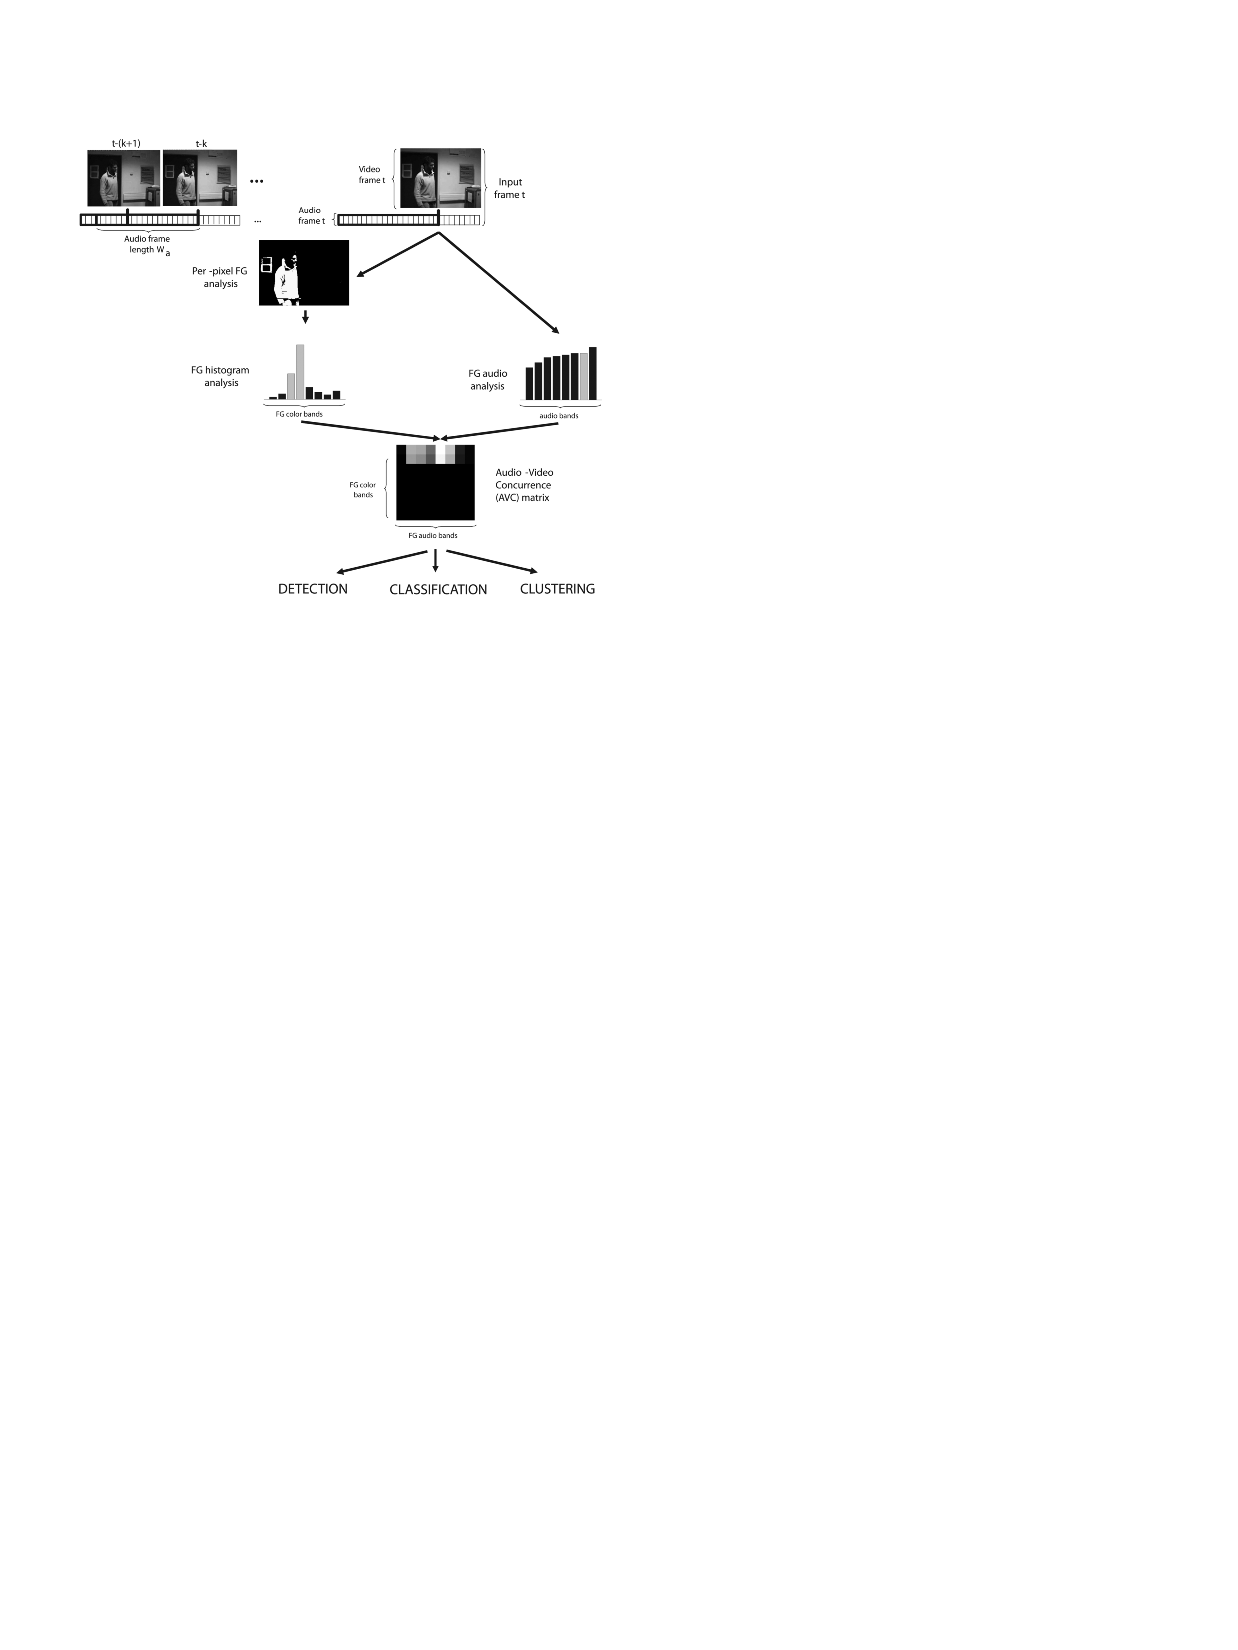
\includegraphics[width=\linewidth]{\figdir/AVC-Overview.pdf}
\caption{Überblick über den Ablauf der AVC Matrix Analyse}
\label{FIG:AVC:Overview}
\end{figure}

\subsection{Zeitadaptive Kombination von Gaußverteilungen}\label{ss:TAPPMOG}

Die Zeitadaptive Kombination von Gaußverteilungen (Time-Adaptive Mixture of Gaussians, kurz TAPPMOG) ist eine Methode zur Erkennung von Abweichungen eines Signals von einem erwarteten Wert mit der Fähigkeit den erwarteten Wert an permanente Veränderungen anzupassen. Somit eignet es sich zum Beispiel für Video-Vordergrund/Hintergrund Analysen, da unerwartete Veränderungen als Vordergrund erkannt werden, aber erwartete Veränderungen, wie das Bewegen eines Baumes im Wind, als Hintergrund. Außerdem werden permanente Veränderungen, wie ein neu abgestelltes Fahrzeug, zunächst als Vordergrund markiert, jedoch über einen kurzen Zeitraum Teil des Hintergrundes. Diese Methode wird im Rahmen der AVC-Matrix Methode sowohl für Video- als auch für Audioanalyse verwendet.  

Das Signal wird mit einer Kombination von \textit{R} Gaußverteilungen modelliert. Dadurch ergibt sich die Wahrscheinlichkeit \textit{P} den Zustand \textit{z\textsuperscript{t}} zum Zeitpunkt \textit{t} zu beobachten wie folgt:

\begin{equation}
P(z^{(t)}) = \sum\limits_{r=1}^R w_r^{(t)} * \mathcal{N}(z^{(t)} | \mu _r^{(t)}, \sigma _r^{(t)})
\end{equation}

Wobei $\mathcal{N}$ eine Gaußverteilungen mit Gewichtung $w_r^{(t)}$, Durchschnitt $\mu _r^{(t)}$ und Standardabweichung $\sigma _r^{(t)}$ ist. All diese Variablen verändern sich im Laufe der Zeit und sind somit von $t$ abhängig. Die Summe der Gewichte alle Gaußverteilungen muss immer eins ergeben.  

Die Gaußverteilungen werden zunächst absteigend nach Gewichtung $w$ sortiert. Die ersten Gaußverteilungen sind die ``erwarteten'' Werte beziehungsweise ``der Hintergrund''. Wird ein neuer Zustand $z$ gemessen, wird er nacheinander gegen jede Gaußverteilung $G_1$ bis $G_R$ geprüft. Ist dieser Wert nicht mehr als $2.5\sigma_i$ vom Durchschnitt $\mu_i$ entfernt, so gilt die Gaußverteilung $G_i$ als Treffer. Anschließend werden die Paramter der Gaußverteilung $G_i$ wie folgt geändert:

\begin{enumerate}

\item Ist $G_i$ ein Treffer
	\begin{itemize}
	\item Erhöhe die Gewichtung $w_i$ (siehe Gleichung \ref{eq:weigth}
	\item Nähere den Durchschnitt $\mu_i$ an $z$ an (siehe Gleichung \ref{eq:mu}
	\item Verringere die Standardabweichung $\sigma_i$ (siehe Gleichung \ref{eq:sigma}
	\item Summiere alle Gewichte der bereits überprüften Verteilungen $G_1, ..., G_i$. Ist die Summe größer als der festgelegte Schwellwert $T$, markiere $z$ als Vordergrund.
	\end{itemize}
\item Ist $G_i$ kein Treffer
	\begin{itemize}
	\item Verringere die Gewichtung $w$ (siehe Gleichung \ref{eq:weigth}
	\end{itemize}
\item Ist keine Gaußverteilung ein Treffer
	\begin{itemize}
	\item Markiere $z$ als Vordergrund
	\item Entferne die Letzte Gaußverteilung in der Liste
	\item Füge eine neue Gaußverteilung hinzu mit $\mu = z$, einer hohen Varianz $\sigma$ und einer geringen Gewichtung $w$
	\end{itemize}

\end{enumerate} 

Die Veränderung der Gewichtung $w$ erfolgt mit folgender Gleichung:

\begin{equation}
\label{eq:weigth}
w_r^{(t)} = (1-\alpha) * w_r^{(t-1)} + \alpha * M^{(t)}
\end{equation}

wobei $M^{(t)} = 1$ wenn die Gaußverteilung ein Treffer ist, andernfalls gilt $M^{(t)} = 0$. Anschließend müssen alle Gewichte normalisiert werden, dass sie in Summe eins ergeben. Je größer die Lernrate $\alpha$ ist, desto schneller passt sich das Modell an Veränderungen an.  

$\alpha$ ist wie $T$ ein konfigurierbarer Wert und sollte an die Besonderheiten der Aufnahmen angepasst werden.  

Die Standardabweichung und Durchschnitt für Treffer wird mit folgenden Gleichungen angepasst:
\begin{equation}
(siehe Gleichung \ref{eq:mu}
\mu_{r_{treffer}}^{(t)} = (1-p)\mu_{r_{treffer}}^{(t-1)} + pz^{(t)}
\end{equation}
\begin{equation}
(siehe Gleichung \ref{eq:sigma}
\sigma_{r_{treffer}}^{2(t)} = (1-p)\sigma_{r_{treffer}}^{2(t-1)} + p (z^{(t)} - \mu_{r_{treffer}}^{(t)})^T (z^{(t)} - \mu_{r_{treffer}})
\end{equation}

mit $p = \alpha * \mathcal{N}(z^{(t)} | \mu_{r_{treffer}}^{(t)}, \sigma_{r_{treffer}}^{(t)} )$, wobei $\alpha$ wie in Gleichung \ref{eq:weigth} die Lernrate ist.

Es ist eine sogenannte Bootstrap Phase notwendig, in der das Modell den Hintergrund ``lernt''. Anschließend kann es unerwartete Ereignisse erfolgreich als Vordergrund markieren. Die Dauer der Bootstrap Phase ist unter anderem von der Größe der Lernrate $\alpha$ abhängig.

\subsection{Videoanalyse}

Die Videoanalyse besteht aus zwei separaten Modulen. Das erste extrahiert Vordergrundaktivität auf Pixelebene während das zweite Modul durch ein Farben-Histogramm neu erscheinende Objekte identifiziert, siehe Abbildung \ref{FIG:AVC:Overview}.

Die Vordergrunderkennung verwendet das in \ref{ss:TAPPMOG} beschriebene TAPPMOG Verfahren, wobei jedes Pixel $z_n^{(t)}$ einzeln von einem TAPPMOG Modell beschrieben wird. Dargestellt wird ein Pixel als Vektor bestehend aus seinen RGB Werten. Somit wird jedes Pixel unabhängig von allen anderen Pixeln entweder als Vordergrund oder Hintergrund eingestuft.

In einer Videoaufnahme, in welcher ein Baum im Wind weht, wird das selbe Pixel abwechselnd grün sein, wenn die Blätter des Baumes zu sehen sind oder blau, wenn die Blätter zur Seite geweht wurden und der dahinter liegende Himmel zu sehen ist. Nach einer kurzen Trainingszeit (Bootstrapping Phase) wird das TAPPMOG Modell eine Gaußverteilung für grün und eine für blau mit hoher Gewichtung beinhalten und weder grüne noch blaue Pixel werden als Vordergrund markiert. Ändert sich jedoch die Farbe des Pixels auf zum Beispiel Rot weil eine Person mit roter Kleidung in der Kameraaufnahme erscheint, wird entweder keine Gaußverteilung als Treffer markiert oder die Summe der Gewichte ist größer als der Schwellwert $T$ und somit wird das Pixel als Vordergrund markiert. Bleibt die Person dort lange Zeit stehen wird sich das Modell anpassen, einen roten Wert erwarten und das Pixel nicht länger als Vordergrund markieren. Die Dauer hierfür ist von der Lernrate $\alpha$ abhängig, welche in dem in \cite{CBM07} vorgestellten Verfahren für alle Pixel und auch Audio Analysen identisch ist.

Das zweite Modul verwendet die Daten der Vordergrunderkennung um das Erscheinen und Verschwinden von Objekten in den Videoaufnahmen zu erkennen. Hierfür werden alle als Vordergrund markierte Pixel für jeden Zeitschritt $t$ in ein Video Vordergrund Histogramm (VVGH) mit $J$ Säulen unterteilt, wobei jede Säule $v_j^{(t)}$ einen Ausschnitt des Farbspektrums (oder einer Grauskala) repräsentiert. Nun wird jede Säule mit einem eigenen TAPPMOG Modell (siehe \ref{ss:TAPPMOG}) analysiert um unerwartete Veränderungen zu erkennen. Eine neu erscheinende Person in einer sonst nur aus Hintergrund bestehenden Szene wird als Vordergrund markiert, wodurch die Anzahl der Vordergrundpixel im VVGH unerwartet erhöht wird. Daraus lässt sich das Erscheinen eines neuen Objektes erkennen. Bewegt sich die Person einige Zeit in der Szene ist sie weiterhin teil des Vordergrundes, aber das TAPPMOG Modell der VVGH Säulen haben sich an den neuen Wert angepasst und markieren keine Vordergrundaktivität. Verlässt die Person nun die Szene sinkt die Anzahl der Vordergrundpixel. Daraus lässt sich das Verschwinden eines Vordergrund-Objektes erkennen.    

Dieses Verfahren hat den Vorteil, dass es Objekte und Personen unabhängig von der Position in der Szene identifiziert. Es hat jedoch den nachteil, dass Objekte lediglich anhand der Farbe erkannt werden, wodurch zwei gleichfarbige Objekte nicht unterschieden werden können. 

\subsection{Audioanalyse}

Die Audioanalyse basiert darauf die zeitliche Veränderung der Energiewerte einzelner Frequenzbereiche zu analysieren. Diese Energiewerte erlauben die Erkennung und Klassifizierung von akustischen Ereignissen \cite{Pel:CASR}.

Dafür werden die Audioaufnahmen in überlappende Zeitfenster der Länge $W_a$ unterteilt, wobei jedes Zeitfenster für den Zeitpunkt $t$ am $t$en Videoframe endet, wie in Abbildung \ref{FIG:AVC:Overview} zu sehen ist. Für jedes Zeitfenster werden mit dem Yule-Walker Autoregressionsverfahren \cite{Mar:DSA} die Energiewerte (in dB) $X^{(t)}(f_n)$ für $n = 1, ..., N$ berechnet, wobei $f_n$ die Frequenz in Herz ist. Die maximale Frequenz ist $f_N = F_s / 2$ wobei $F_s$ die Samplingrate der Aufnahme ist. Die Genauigkeit der Analyse ist Abhängig von der Anzahl an Frequenzen $N$ und der Zeitfensterlänge $W_a$.

Für jedes Zeitfenster wird die \textit{Zeitfenster Energiemenge} (ZEM) berechnet, welche das Histogramm in Abbildung \ref{FIG:AVC:Overview} repräsentiert. Diese Energiemenge wird in $I$ Frequenzbereich unterteilt, wobei jede Untermenge $a_1, ..., a_I$ eine Säule des Histogramms darstellt. Für jede Säule wird ein eigenes TAPPMOG Model trainiert um ``unerwartete'' Werte und damit den akustischen ``Vordergrund'' zu erkennen. Die ZEM ist ausreichend aussagekräftig um Audio-Vordergrund zu erkennen und Ereignisse zu klassifizieren \cite{Row:OMSS}.

\subsection{Audio-Video-Kombination}

Nun soll ein Zusammenhang zwischen Audio und Video Vordergrund hergestellt werden. Hierfür werden die Säulen $a_1, ..., a_I$ des Audio-Histogramms und die Säulen $v_1, ..., v_J$ des Video-Histogramms zum Zeitpunkt $t$ kombiniert. Ein \textit{Audio Vordergrund Muster} $A_i^{(t_{init}^A, t_{end}^A)}$ in Relation zum Zeitpunkt $t$ ist folgendermaßen definiert:
\begin{equation}
A_i^{(t_{init}^A, t_{end}^A)} = [a_i^{(t_{init}^A)}, a_i^{(t_{init}^A+1)}, ..., a_i^{(t)}, ..., a_i^{(t_{end}^A)} ]
\end{equation}
wobei $\forall t \in [t_{init}^A, t_{end}^A], a_i^{(t)} \in Vordergrund$ gelten muss. Ein \textit{Audio Vordergrund Muster} ist somit eine Reihe von zeitlich aufeinanderfolgenden Werten vom $a_i^{(t)}$, welche alle als Vordergrund eingestuft wurden. Auf diese Art können auch \textit{Video Vordergrund Muster} $V_i^{(t_{init}^V, t_{end}^V)}$ definiert werden.

Eine zeitliche Überlappung (\textit{PRI}) zweier Vordergrund Muster $A_i^{(t_{init}^A, t_{end}^A)}$ und $V_i^{(t_{init}^V, t_{end}^V)}$ lässt sich folgendermaßen berechnen:
\begin{equation}
t_{init}^{AV} = max(t_{init}^A, t_{init}^V)  
\end{equation}
\begin{equation}
t_{end}^{AV} = min(t_{end}^A, t_{end}^V)
\end{equation}
Wenn $t_{init}^{AV} < t_{end}^{AV}$ geil, kann die PRI beschrieben werden als:
\begin{equation}
PRI_{i, j}^{(t_{init}^{AV}, t_{end}^{AV})} = [t_{init}^{AV},t_{init}^{AV}]
\end{equation}
$PRI_{i, j}^{(t_{init}^{AV}, t_{end}^{AV})}$ ist ein Zeitintervall in welchem die Audiosäule $a_i$ und die Videosäule $v_j$ gleichzeitig als Vordergrund markiert sind. Die Gewichtung der AV Kombination ist definiert als 
\begin{equation}
w_{AV}^{(t)}(i, j) = \frac{w_{A, i, q}^{(t)} + w_{V, j, u}^{(t)}}{2} 
\end{equation}
für $t \in PRI_{i, j}^{(t_{init}^{AV}, t_{end}^{AV})}$ (ansonsten gilt $w_{AV}^{(t)}(i, j) = 0$). $w_{V, j, u}^{(t)}$ beziehungsweise $w_{A, i, q}^{(t)}$ sind die Gewichte der Gaußverteilungen für die Videosäule $v_j(t)$ beziehungsweise Audiosäule $a_i(t)$ in den jeweiligen TAPPMOG Modellen, wie in Abbildung \ref{FIG:AVC:Coupling} zu sehen ist.

\begin{figure}
\centering
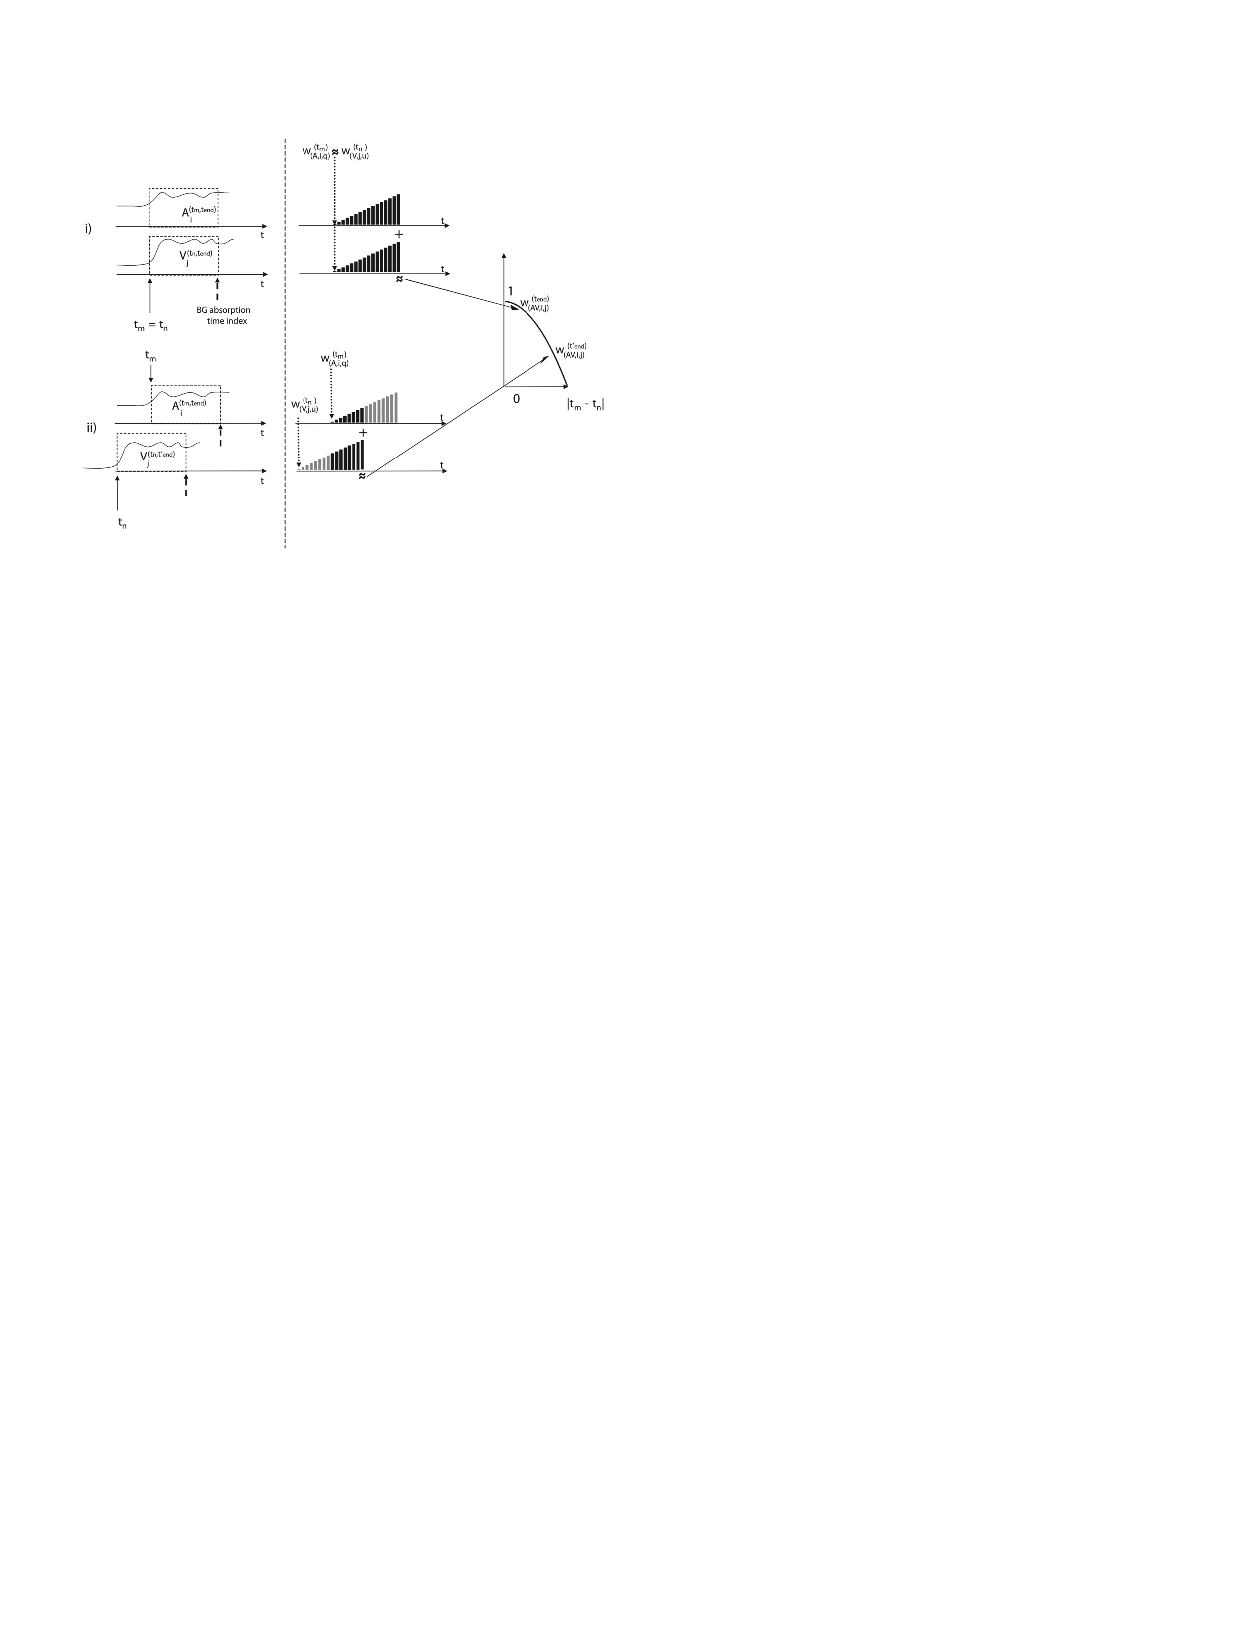
\includegraphics[width=\linewidth]{\figdir/AVC-Coupling.pdf}
\caption{Darstellung des Audio-Video-Kombinationsverfahren. Zeile (i) zeigt zwei stark synchrone Ereignisse während (ii) zwei zeitlich verschobene Ereignisse zeigt. In der Linken Spalte sind die Vordergrund Muster für Audio und Video zu sehen. Die Markierung l für den ``BG absorption time index'' zeigt den Zeitpunkt ab welchem sich das System an das Vordergrund Ereignis angepasst hat und es als Hintergrund kategorisiert. Rechts der gestrichelten Linie sind die Gewichte der Gaußverteilungen der Vordergrundmuster. Das Diagramm rechts zeigt die Kombinationsgewichtung: Je synchroner die Ereignisse sind, desto höher ist ihre Gewichtung}
\label{FIG:AVC:Coupling}
\end{figure}

Aus diesen Daten wird die AVC Matrix erstellt. Diese $I * J$ große Matrix beschreibt den zeitlichen Verlauf vom Zeitpunkt 0 bis $t$ folgendermaßen:
\begin{equation}
AVC^{(t)}(i, j) = \sum\limits_{t'=0}^t w_{AV}^{(t')}(i,j)
\end{equation}

Der Eintrag $[i, j]$ in der AVC Matrix ist die Summe aller bisherigen Audio-Video-Kombinationsgewichtungen für die Audiosäule $a_i$ und die Videosäule $v_j$. Somit ist die Matrix zum Zeitpunkt $t = 0$ leer und wird mit jedem neuen Zeitschritt aktualisiert.

\subsection{Event Erkennung}

Ein \textit{audiovisuelles Event} (AVE) ist im Sinne der AVC Matrix Analyse definiert als ein Zeitintervall, in dem sowohl Audio als auch Video Vordergrund festgestellt wurde. Eine Kombination der Audiosäule $a_i$ und der Videosäule $v_j$ existiert dann, wenn die AVC Matrix an den Koordinaten $[i, j]$ einen nicht-null Wert enthält. Ein AVE existiert dann im Zeitintervall $[t_{init}^{AV}, t_{init}^{AV}]$, wenn folgendes gilt:
\begin{equation} \label{eq:no-pre-sync}
AVC^{(t_{init}^{AV} - 2)} - AVC^{(t_{init}^{AV} - 1)} = 0
\end{equation}
\begin{equation} \label{eq:event-sync}
\forall t \in [t_{init}^{AV}, t_{init}^{AV}], AVC^{(t)} - AVC^{(t + 1)} \neq 0
\end{equation}
\begin{equation} \label{eq:no-post-sync}
AVC^{(t_{end}^{AV} + 1)} - AVC^{(t_{end}^{AV})} = 0
\end{equation}

Gleichung \ref{eq:no-pre-sync} besagt, dass vor Beginn des Events die AVC Matrix unverändert sein muss (also darf kein Audio- und Video-Vordergrund synchron existieren). Die Gleichung \ref{eq:event-sync} besagt, dass während des Zeitintervalls $[t_{init}^{AV}, t_{init}^{AV}]$ durchgehend synchron Audio- und Video-Vordergrund existieren muss und somit bei jedem Zeitschritt mindestens ein Wert der AVC Matrix erhöht wird. Die Gleichung \ref{eq:no-post-sync} besagt, dass nach Ende des Events keine weitere Synchronität zwischen Audio- und Videovordergrund bestehen darf. 

Nun wird für ein AVE $k$ eine \textit{Audio Video Beschreibung} (AVB) erstellt. Diese wird aus der AVC Matrix extrahiert
\begin{equation}
AVB(AVE_k) = AVC^{(t_{end}^{AV}(k))} - AVC^{(t_{init}^{AV}(k)-1)}
\end{equation}

Die AVB enthält die AV Informationen, welche während des Events $k$ gesammelt wurden. Diese Information wird vektorisiert und kann zur Identifizierung von audiovisuellen Events verwendet werden, wie in \ref{ss:experiment} gezeigt wird.

\subsection{Experimentelle Ergebnisse} \label{ss:experiment}

Um die Aussagekräftigkeit der in dieser Methode gewählten AV Eigenschaften zu testen, wurde sie in \cite{CBM07:Experiment} anhand von echten Kameraaufnahmen getestet. Hierbei ist entscheidend, dass die Methode die Events nicht zu allgemein oder zu spezifisch kategorisiert und somit Ergebnisse ähnlich wie ein menschlicher Analyst liefert.

Die Testdaten stammen aus einem Büro und enthalten einzelne Events. Die Events bestehen aus alltäglichen Büroaktivitäten, wie zum Beispiel das Büro betreten oder verlassen, einen Telefonanruf entgegennehmen oder das Bürolicht ein- oder ausschalten (siehe Abbildung \ref{FIG:AVC:TestData}). Die einzelnen Events ereignen sich in einem Abstand von 0.5 bis 10 Sekunden. Die Events überlappen sich nicht, somit ist ein Event immer vollständig abgeschlossen, bevor ein neues beginnt. Es wurden zwei Datensets mit jeweils einer Länger von über zwei Stunden aufgenommen, wobei die aufgenommene Person für das zweite Datenset mehrfach die Kleidung wechselte um die Varianz zu erhöhen.

\begin{figure}
\centering
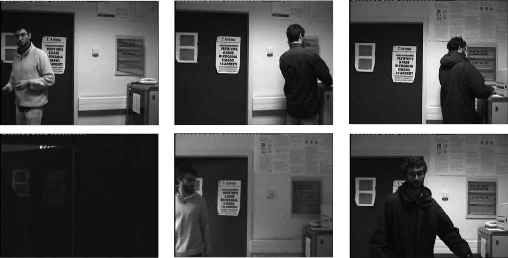
\includegraphics[width=\linewidth]{\figdir/AVC-TestData.pdf}
\caption{Aufnahmen aus den Testdaten}
\label{FIG:AVC:TestData}
\end{figure}

Die Videos wurden mit einer 320x240 CCD Kamera mit 20 Bildern pro Sekunde aufgenommen. Die Audioaufnahmen wurde mit 22050Hz erstellt und in Zeitfenster der Länge $W-a = 1s$ mit einer zeitlichen Überlappung von 70\% unterteilt.   
Für die Anzahl $I$ und $J$ der Audio- und Videosäulen in den Histogrammen wurde $I = J = 8$ gewählt. Versuche zeigten, dass diese Parameter ab einer Größe von 32 zu Performance Problemen führen. Der Wert 8 erlaubt es alle Berechnungen nahezu in Echtzeit durchzuführen mit einem Pentium III 500MHz Prozessor in MATLAB und gleichzeitig eine ausreichende Genauigkeit zu liefern.   

Die Audioaufnahmen wurden in $I = 8$ gleichgroße Abschnitte zwischen $[0, 22050/4]hz$ unterteilt. Für jeden Abschnitt (ein Abschnitt entspricht einer Säule des Histogramms) wurde eine Kombination von drei Gaußverteilungen gewählt (siehe  \ref{ss:TAPPMOG}). Diese Anzahl ist für den einfachen Aufbau der Szenen in den Testdaten ausreichend. Für den Schwellwert $T$ wurde 0.8 gewählt und für die Lernrate $\alpha$ 0.001. Die initiale Gewichtung der Gaußverteilungen für alle TAPPMOG Modelle ist $w_{init} = 0.001$. Diese Werte wurden durch einige initiale Testdurchläufe als akzeptable befunden.

Die Videoaufnahmen werden um den Faktor vier komprimiert, bevor die Vordergrunderkennung auf Pixelebene jeweils mit einem TAPPMOG Modell mit drei Gaußverteilungen durchgeführt wird. Der Vordergrund wird anschließend in ein Histogramm mit $J = 8$ Säulen umgewandelt. Jede Säule stellt einen gleichgroßen Teil des Grauspektrums $[0, 255]$ dar. Für jede Säulen wird ein TAPPMOG Modell mit drei Gaußverteilungen verwendet. Für die Vordergrunderkennung und Histogrammanalyse  wird der gleiche Schwellwert $T$ verwendet, jedoch eine andere initiale Standardabweichung $\sigma_{init}$ für neu initialisierte Gaußverteilungen (siehe \ref{ss:TAPPMOG} Fall 3. ``Keine Gaußverteilung ist ein Treffer''), da sich die Zahlenintervalle stark unterscheiden.

Die Größe der Standardabweichung stellte sich als entscheidend für die AVC Methode heraus. Bei einem zu geringen Wert deckten mehrere Gaußverteilungen gleiche Muster ab, wodurch andere Hintergrundmuster fälschlicherweise als Vordergrund markiert wurden. Bei einer zu großen Standardverteilung ist die Gefahr groß, dass eine Gaußverteilung mehrere verschiedene Muster gleichzeitig abdeckt.   
Nach der Analyse mehrere Konfigurationen wurden folgende Werte für die initialen Standardabweichungen verwendet:
\begin{enumerate}
\item $\sigma_{init}^A = 10$ für die Audioanalyse (ZEM Wert im Bereich $[0, 150]$)
\item $\sigma_{init}^P = 30$ für die Pixel-Vordergrundanalyse (Pixelsignal im Bereich $[0, 255]$)
\item $\sigma_{init}^V = 50$ für die Videohistogramm-Analyse (VVGH Werte im Bereich $[0, 4800]$
\end{enumerate}

In Abbildung \ref{FIG:AVC:Example} ist der Ablauf eines AV Events AVE zu sehen. Nach dem Ende des AVEs kann die AV Beschreibung AVB als Vektor aus der Veränderung der AVC Matrix berechnet werden. Dieser AVB Vektor wird als Eingabe für Klassifizierung und Clustering verwendet.

Die kompletten vier Stunden Testdaten wurden zunächst von einem menschlichen Analysten bewertet, welcher 66 AVEs erkannte. Diese wurden kategorisiert in folgende Ereignisse:
\begin{enumerate}
\item \textit{Anruf tätigen}: Eine Person bewegt sich zum Telefon, wählt eine Nummer und führt ein Gespräch
\item \textit{Anruf erhalten}: Das Telefon klingelt, eine Person bewegt sich zum Telefon, hebt ab und führt ein Gespräch
\item \textit{Ankunft (erster)}: Eine Person betritt das dunkle Labor, schaltet das Licht an und betritt den Raum ohne zu sprechen.
\item \textit{Ankunft (nicht erster)}: Eine Person betritt den beleuchteten Raum und spricht
\item \textit{Verlassen (letzter)}: Eine Person verlässt das Labor ohne zu sprechen und schaltet das Licht aus
\item \textit{Verlassen (nicht letzter)}: Eine Person verlässt das Labor und spricht
\end{enumerate}


\begin{figure} 
\centering
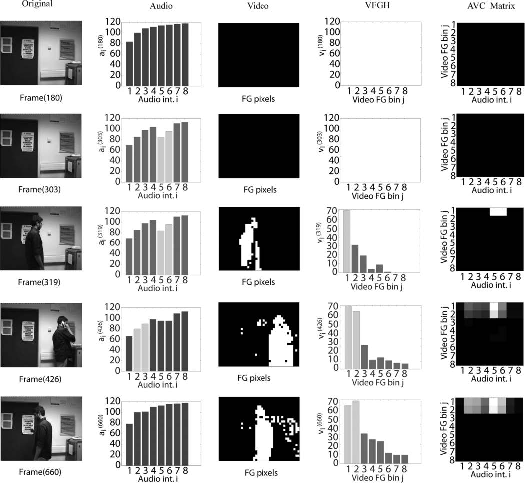
\includegraphics[width=\linewidth]{\figdir/AVC-Example.pdf}
\captionsetup{singlelinecheck=off}
\caption[foo bar]{Beispiel: ``Anruf erhalten'' Event.  Das Telefon im Bild klingelt, eine Person betritt das Bild, beantwortet den Anruf und verlässt danach das Bild. Jede der fünf Zeilen enthält einen Frame und dessen AVC Matrix Analyse:
\begin{enumerate}
\item Frame 180: Keine Aktivität, der Hintergrund ist etabliert
\item Frame 303: Das Telefon klingelt und verursacht Audiovordergrund (Balken 5 \& 6 im Audiohistogram). Da jedoch kein Videovordergrund erkannt wurde bleibt die AVC Matrix leer.
\item Frame 319: Eine Person betritt das Bild und wird als Vordergrund erkannt. Die Kombination aus Vordergrund in der Videosäule 1 und den Audiosäulen 5 \& 6 erzeugt Einträge in der AVC Matrix an Position [5,1] und [6,1]. Der Anfang es AV Event wird erkannt.
\item Frame 426: Die Person spricht am telefon und die AVC Matrix wird weiter befüllt.
\item Frame 660: Die Person hat das Gespräch beendet. Da kein Audiovordergrund mehr existiert bleibt die AVC Matrix unverändert und das Ende des AV Events wird erkannt.
\end{enumerate}
}
\label{FIG:AVC:Example}
\end{figure}

Um die Klassifizierungsgenauigkeit der AVC Matrix Analyse zu bewerten, wurden folgende Szenarien genauer untersucht:
\begin{itemize}
\item Szenario A - Situation 1 und 2 unterschieden (Anruf tätigen / erhalten)
\item Szenario B - Situation 3 und 4 unterscheiden (Leeres / nicht-leeres Labor betreten)
\item Szenario C - Situation 5 und 6 unterscheiden (Leeres / nicht-leeres Labor verlassen)
\item Szenario D - Alle Situationen unterscheiden
\end{itemize}

Die Klassifizierung wurde mit dem KNN Algorithmus (Euklidische Distanz) berechnet \cite{KNN:KNN}. Dies ist ein simpler Klassifizerungsalgorithmus, erlaubt es jedoch die Aussagekräftigkeit von Eigenschaften zu bewerten. Die Bewertung der Ergebnisse wurde mit dem ``Leave-One-Out'' (LOO) Verfahren durchgeführt \cite{KNN:KNN}. Die Klassifizierung anhand der AVC Matrix wurde verglichen mit der Klassifizierung anhand des Audio- beziehungsweise Videovordergrund alleine. Hierfür wurde die Klassifizierung statt mit dem Vektor der AVB aus der AVC Matrix direkt mit dem Vektor aus dem Audio- beziehungsweise Video-Histogramm durchgeführt.    

Die Audioanalyse ist sehr effektiv in Szenario A, da das Erhalten eines Anrufes anhand des Klingelgeräusches deutlich vom Tätigen eines Anrufes zu unterscheiden ist. Die reine Videoanalyse liefert in Szenario B und C ein zufriedenstellendes Ergebnis, da sich die Situationen durch die an- beziehungsweise ausgeschaltete Beleuchtung visuell stark unterscheiden. In jedem Fall ist die Verwendung der AVC Matrix, statt nur einer einzelnen Modalität, gleich erfolgreich oder erfolgreicher. Für Szenario D, Kategorisierung aller Situationen, ist die AVC Matrix Analyse sogar etwa 25\% erfolgreicher. Ein wichtiger Vergleich ist noch mit der Leistung der AV Konkatenation (``AV Kon.'' Spalte in Tabelle \ref{FIG:AVC:Evaluate}). Bei dieser Methode werden die Vektoren von Audio und Video zu einem einzelnen Vektor zusammengefasst, ähnlich der in \cite{MJS:MMAV} verwendeten Methode. Auch hier ist die AVC Matrix Analyse erfolgreicher, wodurch gezeigt wird, dass die zeitliche Synchronität der beiden Modalitäten eine nutzbringende Information ist.



\begin{table}
\centering
\caption{Erfolgsquote beim Klassifizieren der Szenarien anhand von Audio, Video oder Audio-Video }
\begin{tabular}{ccccc}
Szenario & Audio & Video & AV Kon. & AVC Matrix \\
\hline
A & 100,00\% & 86,35\% & - & 100,00\% \\
B & 60,87\% & 95,65\% & - & 95,65\% \\
C & 95,24\% & 85,71\% & - & 95,24\% \\
D & 62,12\% & 66,67\% & 82,28\% & 89,39\% \\
\end{tabular}
\label{FIG:AVC:Evaluate}
\end{table}

Zur weiteren Bewertung der Methode wurden die Events hierarchisch, mit euklidische Distanz in Cluster gruppiert \cite{JD:ACD} , wie in Abbildung \ref{FIG:AVC:Clustering} zu sehen ist. An der X-Achse des Diagramms ist die Nummer der Situation des Events zu sehen. Situation 2, 3 und 5 wurden sehr gut erkannt, da diese sehr eindeutige Merkmale besitzen: Ein klingelndes Telefon beziehungsweise das ein- oder ausschalten der Beleuchtung. Situation 4 und 6 sind schwerer unterscheidbar: In Situation 4 gibt es einen AV Vordergrund wenn die Tür geöffnet wird und die Person den Raum betritt. Der anschließende Audiovordergrund beinhaltet das Schließen der Tür und das Sprechen der Person während die Person sich durch die Szene bewegt. In Situation 6 hingegen ist nach dem Schließen der Tür kein Videovordergrund mehr in der Szene vorhanden, wodurch das Schließgeräusch nicht in die AVC Matrix eingerechnet wird.

Die Clustering Genauigkeit wird aus der Anzahl der Ereignisse in falschen Clustern berechnet, wobei die Nummer des Clusters gleich der Nummer der Mehrheit seiner Einträge ist. Somit beträgt die Genauigkeit 75,76\%. Im Vergleich zum reinen Audio Clustering mit 53,03\%, reinem Video Clustering mit 60,61\% und dem Clustering anhand der einfachen Videokonkatenation mit 64,44\% liefert die AVC Matrix Methode ein deutlich genaueres Ergebnis und zeigt, dass die Verbindung der Audio- und Video-Modalitäten und deren zeitliche Synchronität einen höheren Informationsgehalt liefern, als bisherige Methoden.

\begin{figure} 
\centering
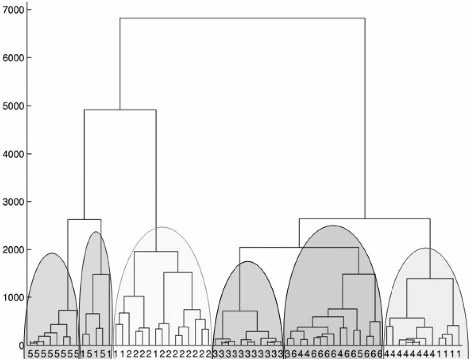
\includegraphics[width=\linewidth]{\figdir/AVC-Clustering.pdf}
\caption{Clustering der Daten in einem Dendrogram}
\label{FIG:AVC:Clustering}
\end{figure}

\section{Alternative Methoden}
\subsection{Mikrofonreihen} \label{ss:array}
Ein System bestehend aus mehreren Mikrofonen und Kameras ermöglicht eine sehr detaillierte Eventerkennung und räumlich Bewegungsverfolgung von Objekten und Personen im überwachten Bereich. Das in \cite{Che02} beschriebene System überwacht einen Konferenzsaal mit 32 ungerichteten Mikrofonen, welche an der Decke des Saales befestigt sind, und zwei Videokameras ähnlich zu der in Abbildung \ref{FIG:Array:Setup} dargestellten Umgebung.

\begin{figure}
\centering
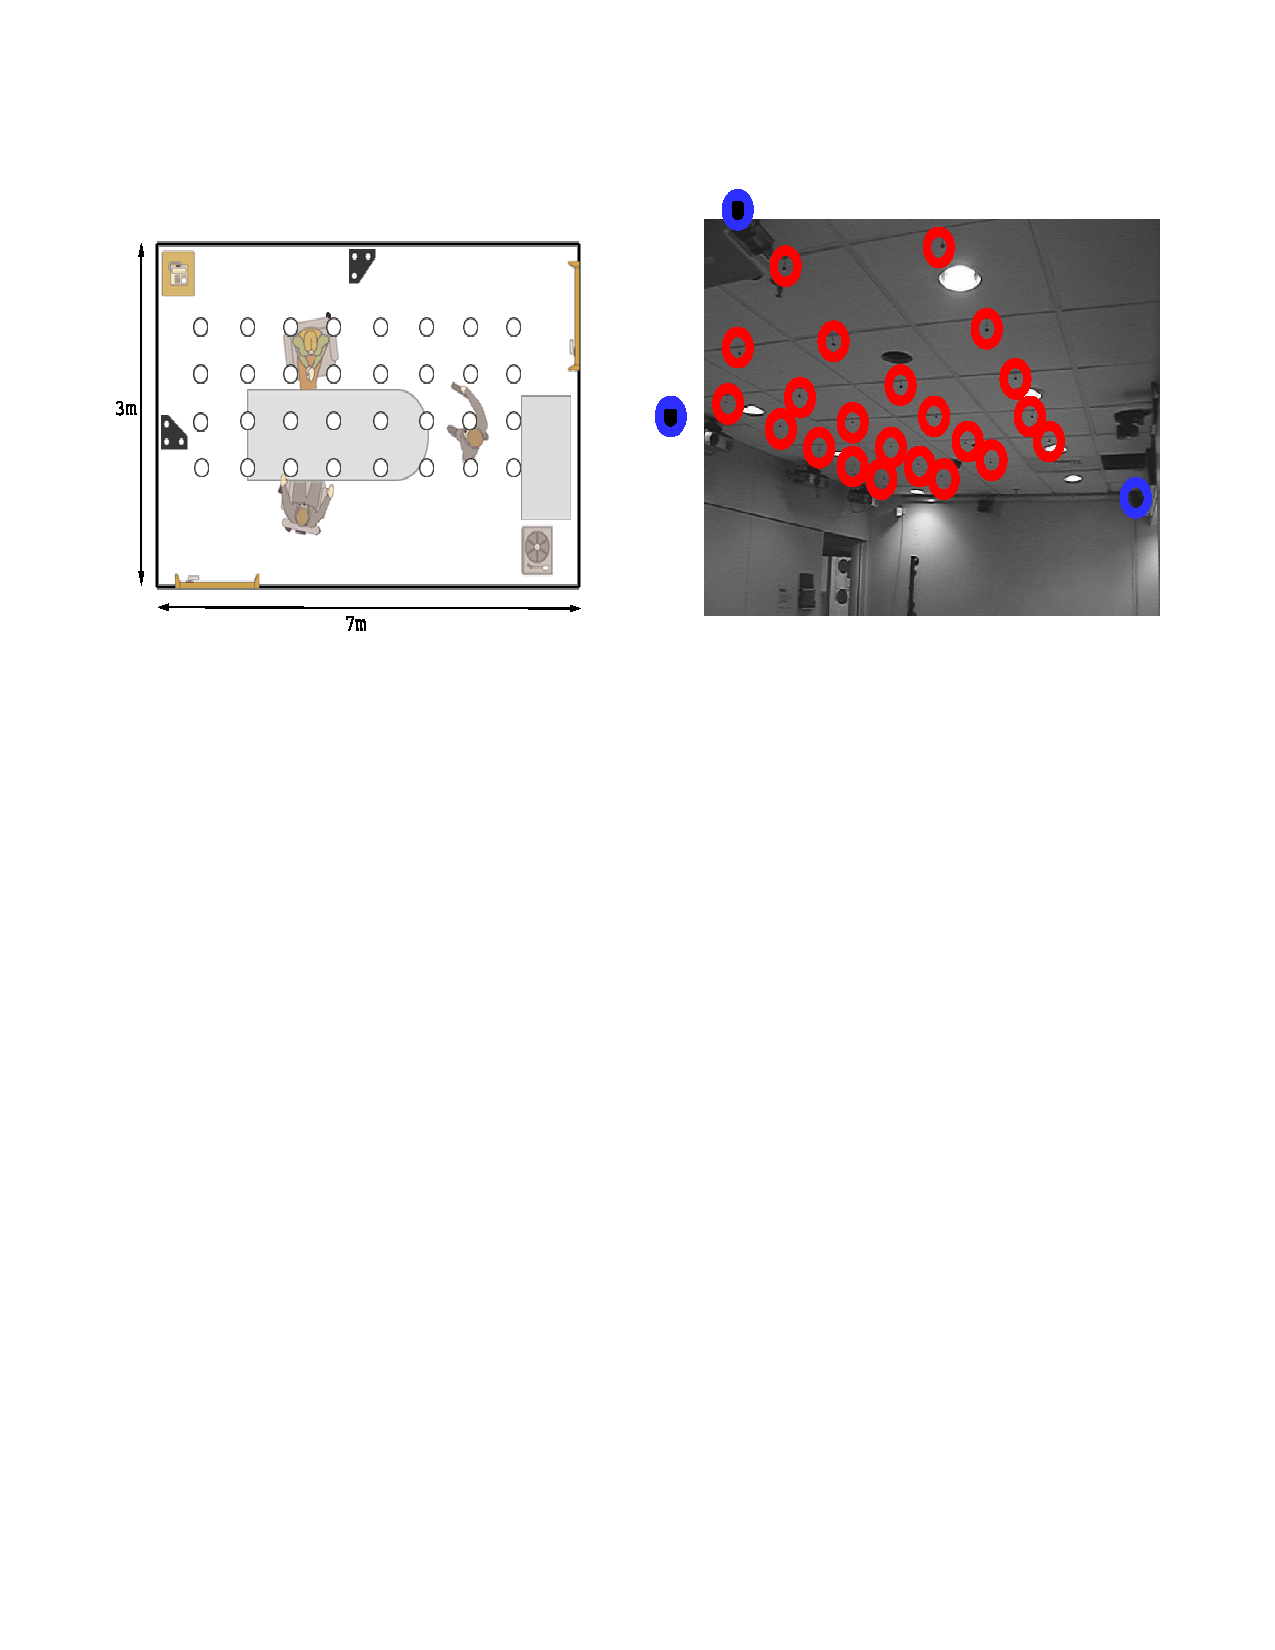
\includegraphics[width=\linewidth]{\figdir//MA-Setup.pdf}
\caption{Links eine schematische Zeichnung, in der die Kreise Mikrofone darstellen und die schwarzen Dreiecke Kameras. Rechts ist ein Foto der Testumgebung in welchem Kameras und Mikrofone hervorgehoben wurden. Quelle \cite{Array:Setup}}
\label{FIG:Array:Setup}
\end{figure}

Die Videoaufnahmen werden mit einer Foreground-Background-Analysis aufbereitet um Veränderungen in den Aufnahmen kenntlich zu machen. Diese Veränderungen im Verhältnis zur Zeit stellen die Bewegungen der Personen in den Videoaufnahmen dar \cite{Array:Video}. Da die Anwendung Personen in einem Konferenzsaal beobachtet, wird die Position lediglich auf eine zweidimensionalen Fläche projiziert. In Abbildung \ref{FIG:Array:Video} ist eine Videoanalyse zu sehen. Die X und Y Achsen geben die Position der Bewegung im Raum an während die Z Achse der zeitliche Verlauf ist. In der Abbildung ist eine Momentaufnahme für t=29 zu sehen. Diese zeigt alle Regionen, in denen zu diesem Zeitpunkt t Bewegungen festgestellt wurden. Insgesamt zeigt die Grafik einen Bewegungsverlauf von zwei Personen, welche sich der Raummitte nähern und einem Objekt in der Raummitte, welches ungefähr ab dem Zeitpunkt t=25 bewegt wird. Nach dem Zeitpunkt t=40 bewegen sich die zwei Personen wieder aus der Mitte des Raumes hinaus.

\begin{figure}
\centering
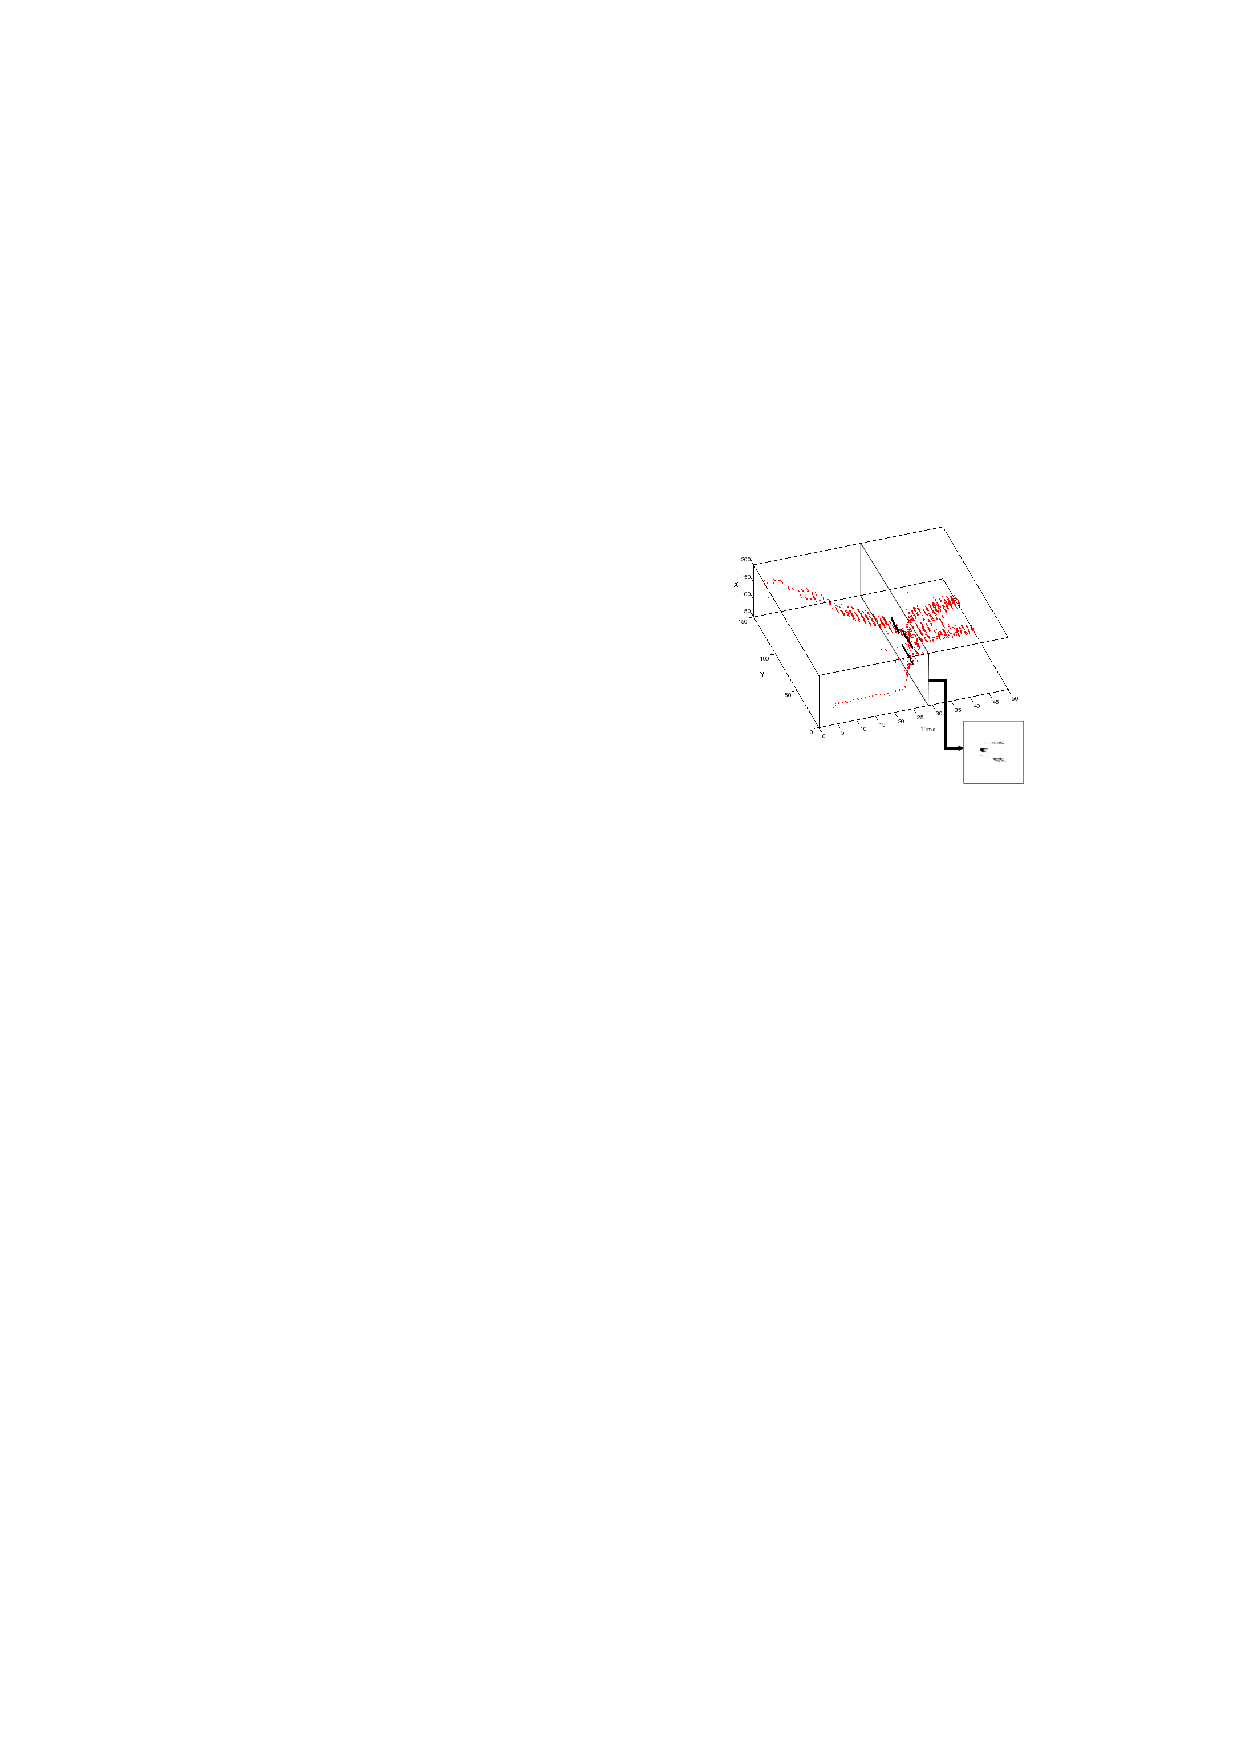
\includegraphics[width=0.75\linewidth]{\figdir//MA-VT.pdf}
\caption{Video Analyse von Bewegungen im Verlauf der Zeit}
\label{FIG:Array:Video}
\end{figure}

Mit den Werten der Mikrofone wird die Lautstärke im Vergleich zu Rauschgeräuschen (SNR, Signal-Noise-Ratio) auf dem Raum abgebildet. Somit wird ein Graph wie in Abbildung \ref{FIG:Array:Audio} erzeugt. Da dieses System eine Gruppe von Menschen beobachtet, arbeitet es unter der Annahme, dass Bewegung und Geräusche korrelieren. Deshalb werden die Positionen, an denen es visuelle Bewegungen gab, als Ausgangspunkt für eine Suche nach einem lokalen Maximum im Audiographen verwendet \cite{Che02:Audio}. Somit kann die genaue Position der Geräuschquelle lokalisiert werden. Mithilfe der Position können die Zeitverzögerungen der Audioaufnahmen der unterschiedlichen Mikrofone berechnet und somit das Zielgeräusch von Hintergrundgeräuschen getrennt werden \cite{Array:Audio}.    

\begin{figure}
\centering

\includegraphics[width=0.8\linewidth]{\figdir//MA-AT.pdf}
\caption{Räumliche Audio Analyse durch mehrere Mikrofone}
\label{FIG:Array:Audio}
\end{figure}

\bigskip

Die Audio- und Videodaten werden zu einem beobachteten Zustand \textit{z} kombiniert. Dann wird berechnet wie wahrscheinlich diese Beobachtung \textit{z} für eine hypothetische Konfiguration \textit{O\textsubscript{t}}
\begin{equation}
O_t = (o_1, ..., o_n)
\end{equation}

aus \textit{n} Objekten zum Zeitpunkt \textit{t} ist, wobei \textit{O\textsubscript{i} = [x, y, h, f]} der Zustandsvektor eines Objektes ist. Hierbei werden Personen als Zylinder der Höhe \textit{h} mit festgelegten Radio dargestellt, dessen Position auf dem Boden durch [\textit{x, y}] dargestellt wird. \textit{f} ist die Frequenz ihrer Stimme.

Für ein einzelnes Objekt gibt \textit{L(z|O\textsubscript{i})} an, wie wahrscheinlich die Hypothese eines einzelnen Objektes von der Beobachtung unterstützt wird. Dies wird berechnet aus

\begin{equation}
L(z|o_i) = L(z_a|o_i) * L(z_v|o_i)
\end{equation}

wobei $L(z_a|o_i)$ und $L(z_v|o_i)$ angeben, wie sehr die Audio- beziehungsweise Videodaten die Hypothese $o_i$ unterstützen.

Die Wahrscheinlichkeit $L_t(z|O)$, dass der beobachtete Zustand für eine Hypothese \textit{O} bestehend aus \textit{m} Objekten auftritt lässt sich mit dem gauschen Fehlintegral aus den Einzelwahrscheinlichkeiten der Objekte berechnen

\begin{equation}
L_t(z|O) = \phi L(z|o_1), ..., L(z|o_m)
\end{equation}

\bigskip

Mikrofonreihen erlauben es selbst sich bewegende Audio-Visuelle Ereignisse mit einer Genauigkeit von bis zu 10 Zentimeter zu erkennen und verfolgen. Somit können auch Gespräche zwischen zwei nahestehenden Personen korrekt erkannt werden. Auch können zwei gleichzeitige, unabhängige AV Events separat erkannt werden. Jedoch benötigt diese Methode eine große Menge an Mikrofonen und Rechenleistung und ist daher nur in sehr kontrollierten Umgebungen einsetzbar \cite{Che02}.

\subsection{Dualmikrofon mit HHM}

\subsection{Cononical correlation analysis}

\subsection{Maximization of mutual information}

\subsection{Computational Auditory Scene Analysis CASA}
\subsection{Computational Auditory Scene Recognition CASR}

\section{Bewertung} 

Die AVC Matrix Methode ist eine neue Methode um audiovisuelle Eventerkennung für Videoaufnahmen mit einer Kamera und einem Mikrofon zu automatisieren. Die Video- und Audiosignale werden separat mit adaptiven Modellen verarbeitet, um Vordergrund und Hintergrund zu unterscheiden. Anschließend werden anhand ihrer zeitlichen Synchronität Audio-Video-Events erkannt. Dies wird mit einer Audio-Video-Concurrency (AVC) Matrix berechnet. Die Methode lieferte in den durchgeführten Experimente bessere Ergebnisse, als die Verwendung reiner Audio- oder Videodaten. Auch liefert sie bessere Ergebnisse als die Verwendung von Audio-Video-Daten welche ohne die zeitliche Synchronität kombiniert wurden.

Die Methode verwendet simple Algorithmen für die Videoerkennung, wodurch zum Beispiel mehrere gleichfarbige Objekte nicht unterschieden werden können. Die AVC Matrix Methode kann jedoch auch mit weiterentwickelten Videoanalyse Methoden kombiniert werden. Außerdem ist diese Methode nicht in der Lage mehrere gleichzeitig erscheinende Events korrekt zu trennen.


% \appendix
% \section{Erster Abschnitt des Anhangs}
\label{a:somelabel}
In diesem Anhang wird \dots 

%%% Local Variables: 
%%% mode: latex
%%% TeX-master: "thesis.tex"
%%% End: 



\bibliographystyle{natger}
\bibliography{thesis}



\end{document}
